\scanpage{18}
cette dernière, si $\operatorname{card}J=\operatorname{card}I-1=n-1$, on verra (par \unsure{récurrence}) que le cardinal de l'ens des classes est $(n-1)+1=n$.

Ceci posé, on voit d'abord que $E_i$ est dans
% G01: manual source origin (805,390), full-scan pixels; x right, y down.
% Words l'une, (unique), des/de, ces n occur only in this group.
\begin{tikzpicture}[x=.007cm,y=-.007cm,baseline={(0,178)}]
\path[use as bounding box] (0,75) rectangle (710,205);
\node[anchor=base west,inner sep=0,outer sep=0] at (24,178) {l'une};
\node[anchor=base west,inner sep=0,outer sep=0] at (220,108) {\inserted{(unique)}};
\node[anchor=base west,inner sep=0,outer sep=0] at (286,178) {\unsure{des|de}};
\node[anchor=base west,inner sep=0,outer sep=0] at (452,178) {ces $n$};
% G01.P1: bent insertion guide, including its raised right endpoint.
\draw[line width=.35pt] (283,170) .. controls (270,120) and (321,128) .. (384,124) .. controls (426,124) and (462,114) .. (470,109) -- (470,104);
\end{tikzpicture}
classes, qui sont des ouverts. Soit $U_{J,i}$ la classe (ou ``composante'') qui contient $E_i$, et considérons les deux composantes $\Sigma_i^+,\Sigma_i^-$ de $X\setminus E_i$.

% G02: source origin (225,1145). The two manual rules replace a full-height tabular rule.
\figure{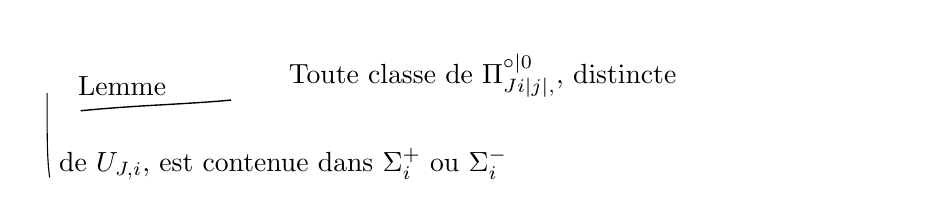
\begin{tikzpicture}[x=.008cm,y=-.008cm]
\path[use as bounding box] (0,0) rectangle (1420,265);
\node[anchor=base west,inner sep=0,outer sep=0] at (80,108) {\rlap{Lemme}\phantom{\uline{Lemme}}};
\node[anchor=base west,inner sep=0,outer sep=0] at (415,88) {Toute classe de $\Pi_{J\deleted{\unsure{i|j|,}}}^{\unsure{\circ|0}}$, distincte};
\node[anchor=base west,inner sep=0,outer sep=0] at (50,229) {de $U_{J,i}$, est contenue dans $\Sigma_i^+$ ou $\Sigma_i^-$};
% G02.P1: single slightly rising underline beneath Lemme.
\draw[line width=.5pt] (84,132) .. controls (174,123) and (248,122) .. (323,115);
% G02.P2: separate left rule starts below the first row and ends beside the second.
\draw[line width=.4pt] (31,104) .. controls (31,151) and (30,207) .. (35,238);
\end{tikzpicture}}

C'est presque une tautologie : Dire
% G03: source origin (220,1475). The following ordinary words classe donnée are outside this group once.
\begin{tikzpicture}[x=.007cm,y=-.007cm,baseline={(0,99)}]
\path[use as bounding box] (0,20) rectangle (215,125);
\node[anchor=base west,inner sep=0,outer sep=0] at (83,99) {\rlap{la}\phantom{\deleted{la}}};
\node[anchor=base west,inner sep=0,outer sep=0] at (20,48) {\inserted{qu'une}};
% G03.P1: complete bent guide, with short right return.
\draw[line width=.35pt] (49,109) .. controls (76,77) and (110,67) .. (158,62) .. controls (176,59) and (195,47) .. (204,40) .. controls (206,36) and (202,35) .. (197,37);
% G03.P2: cancellation through la; no additional generic visible strike.
\draw[line width=.7pt] (85,95) -- (147,83);
\end{tikzpicture}
classe donnée
% G04: source origin (710,1445). U_alpha, de Pi_J, and baseline ne each occur once.
% The hook represented by G04.P2 is C's comma candidate; its punctuation/guide role stays unresolved.
\begin{tikzpicture}[x=.007cm,y=-.007cm,baseline={(0,118)}]
\path[use as bounding box] (0,10) rectangle (330,140);
\node[anchor=base west,inner sep=0,outer sep=0] at (26,68) {\inserted{$U_{\unsure{\alpha|x}}$}};
\node[anchor=base west,inner sep=0,outer sep=0] at (112,53) {\inserted{de $\Pi_J^\circ$}};
\node[anchor=base west,inner sep=0,outer sep=0] at (89,118) {ne};
% G04.P1: rising left guide, bowed middle, and right return.
\draw[line width=.35pt] (49,110) .. controls (49,99) and (79,81) .. (105,68) .. controls (134,59) and (158,89) .. (211,79) .. controls (260,68) and (293,55) .. (301,43) -- (298,40);
% G04.P2: one qualified hook at fixed local origin (98,52), base-west anchored.
\node[anchor=base west,inner sep=0,outer sep=0] at (98,52) {\unsure{\begin{tikzpicture}[x=.007cm,y=-.007cm,baseline=0pt]
\path[use as bounding box] (0,0) rectangle (16,20);
\draw[line width=.45pt] (1,3) .. controls (9,0) and (14,7) .. (7,16);
\end{tikzpicture}}};
\end{tikzpicture}
contient pas $\deleted{\Sigma}\overline{E_i}$ i.e. est $\ne U_{J,i}$, signifie que il existe un $j\in J$ tel que le $\Sigma_j^+\in\pi_0(X\setminus\deleted{\Sigma}E_{\unsure{j|J}})$
% G05: source origin (1405,1720); uncertain word, single literal cancellation, two detached points.
\begin{tikzpicture}[x=.01cm,y=-.01cm,baseline={(0,50)}]
\path[use as bounding box] (0,0) rectangle (190,80);
\node[anchor=base west,inner sep=0,outer sep=0] at (0,50) {\rlap{\unsure{choisi|choisie}}\phantom{\deleted{\unsure{choisi|choisie}}}};
% G05.P1: cancellation run through the word.
\draw[line width=.65pt] (7,39) .. controls (55,40) and (109,41) .. (160,43);
% G05.P2-P3: detached points at fixed local origin (165,32); no character or role supplied.
\node[anchor=base west,inner sep=0,outer sep=0] at (165,32) {\unsure{\begin{tikzpicture}[x=.01cm,y=-.01cm,baseline=0pt]
\path[use as bounding box] (0,-8) rectangle (13,8);
\fill (2,2) ellipse [x radius=1,y radius=1.4];
\fill (8,-5) ellipse [x radius=.9,y radius=1.2];
\end{tikzpicture}}};
\end{tikzpicture}
``composant'' de cette classe \deleted{est} est l'élément du $\pi_0$ qui ne contient pas $E_i$; il est donc contenu dans l'un des
% G06: source origin (240,2080). Complete elements/insert/de group; following pi expression occurs outside once.
\begin{tikzpicture}[x=.007cm,y=-.007cm,baseline={(0,176)}]
\path[use as bounding box] (0,90) rectangle (430,195);
\node[anchor=base west,inner sep=0,outer sep=0] at (30,180) {éléments};
\node[anchor=base west,inner sep=0,outer sep=0] at (155,133) {\inserted{(soit $\Sigma_i^-$)}};
\node[anchor=base west,inner sep=0,outer sep=0] at (351,168) {de};
% G06.P1: insertion guide with small raised right return.
\draw[line width=.35pt] (319,165) .. controls (320,141) and (359,143) .. (405,127) -- (409,124) -- (405,120);
\end{tikzpicture}
$\pi_0(X\setminus\Sigma_i)$, d'après l'étude du cas
% G07: source origin (245,2240); deleted word, raised replacement and comma occur once.
\begin{tikzpicture}[x=.008cm,y=-.008cm,baseline={(0,85)}]
\path[use as bounding box] (135,15) rectangle (335,110);
\node[anchor=base west,inner sep=0,outer sep=0] at (153,85) {\rlap{\unsure{deux}}\phantom{\deleted{\unsure{deux}}}};
\node[anchor=base west,inner sep=0,outer sep=0] at (145,49) {\inserted{$\operatorname{card}I=2$}};
\node[anchor=base west,inner sep=0,outer sep=0] at (300,95) {,};
% G07.P1: long slightly rising cancellation beneath the inserted formula.
\draw[line width=.65pt] (152,86) .. controls (193,79) and (252,84) .. (303,78);
\end{tikzpicture}
\deleted{\unsure{cela|OK}} \unsure{â|à} fortiori $U_\alpha\subset\Sigma_i^-$,
% G08: source origin (1440,2250). OK's rising stroke has unresolved joining/cancellation state.
\begin{tikzpicture}[x=.01cm,y=-.01cm,baseline={(0,55)}]
\path[use as bounding box] (0,0) rectangle (210,95);
\node[anchor=base west,inner sep=0,outer sep=0] at (11,55) {\unsure{\begin{tikzpicture}[x=.01cm,y=-.01cm,baseline=0pt]
\path[use as bounding box] (0,-45) rectangle (85,8);
\node[anchor=base west,inner sep=0,outer sep=0] at (0,0) {\rlap{OK}\phantom{\deleted{OK}}};
% G08.P1: the visible rising crossing/joining stroke, drawn only here.
\draw[line width=.35pt] (0,-15) .. controls (24,-21) and (51,-32) .. (73,-40);
\end{tikzpicture}}};
\node[anchor=base west,inner sep=0,outer sep=0] at (127,61) {.};
% G08.P2: faint detached spot; shape, hand, surface origin and role remain qualified.
\node[anchor=base west,inner sep=0,outer sep=0] at (192,42) {\unsure{\begin{tikzpicture}[x=.01cm,y=-.01cm,baseline=0pt]
\path[use as bounding box] (0,0) rectangle (6,6);
\fill[gray] (2,2) ellipse [x radius=1.1,y radius=1.6];
\end{tikzpicture}}};
\end{tikzpicture}
% archive sheet number: 17
